\section{相关技术基础}
在本节中,我们将介绍图神经网络(GNN)和图形处理单元(GPU)的基础知识以及两种主要的GNN计算框架:基于GPU的图系统和深度学习框架。

\subsection{图神经网络}
图~\ref{fig:gnn-computation-flow}展示了图神经网络在单次迭代中的计算流程。GNN再$k+1$层基于第$k$层($k\geq 0$)的节点嵌入信息,如公式~\ref{eq: GNN}所示:
\begin{gather} \label{eq: GNN}
    \begin{aligned} 
      a_{v}^{(k+1)}  &= \mathbf{Aggregate}^{(k+1)}({h_{u}^{(k)}|u\in \mathbf{N}(v)\cup h_v^{(k)}}) \\
      h_{v}^{(k+1)}  &= \mathbf{Update}^{(k+1)}(a_{v}^{(k+1)})
   \end{aligned}   
\end{gather}
其中,$h_{v}^{(k)}$ 表示节点 $v$ 在第 $k$ 层的嵌入向量;$h_v^{(0)}$ 通过仅用于符号值嵌入空间映射的初始嵌入函数,由节点特定任务特征(如顶点关联的文本或顶点所表征实体的标量属性)计算得出;$a_{v}^{(k+1)}$ 是通过聚合邻居信息(如节点嵌入)得到的聚合结果;$\mathbf{N}(v)$ 表示节点 $v$ 的邻居集合。不同图神经网络在聚合方法与更新顺序上存在差异:部分方法~\cite{GCNConv, SageConv} 只依赖相邻节点信息,而另一些方法~\cite{GATConv} 还会结合边属性——通过计算每条边两端节点嵌入的点积,并融合边特征(边类型及其他属性)来实现。更新函数通常由标准神经网络操作构成,例如采用 $w\cdot a_{v}^{(k+1)} + b$ 形式的全连接层或多层感知机(MLP),其中 $w$ 和 $b$ 分别为可学习的权重和偏置参数。节点嵌入向量的维度常见取值为16、64和128,不同层间的嵌入维度可能发生变化。
\begin{figure}[htbp] % 调整浮动位置参数
    \centering
    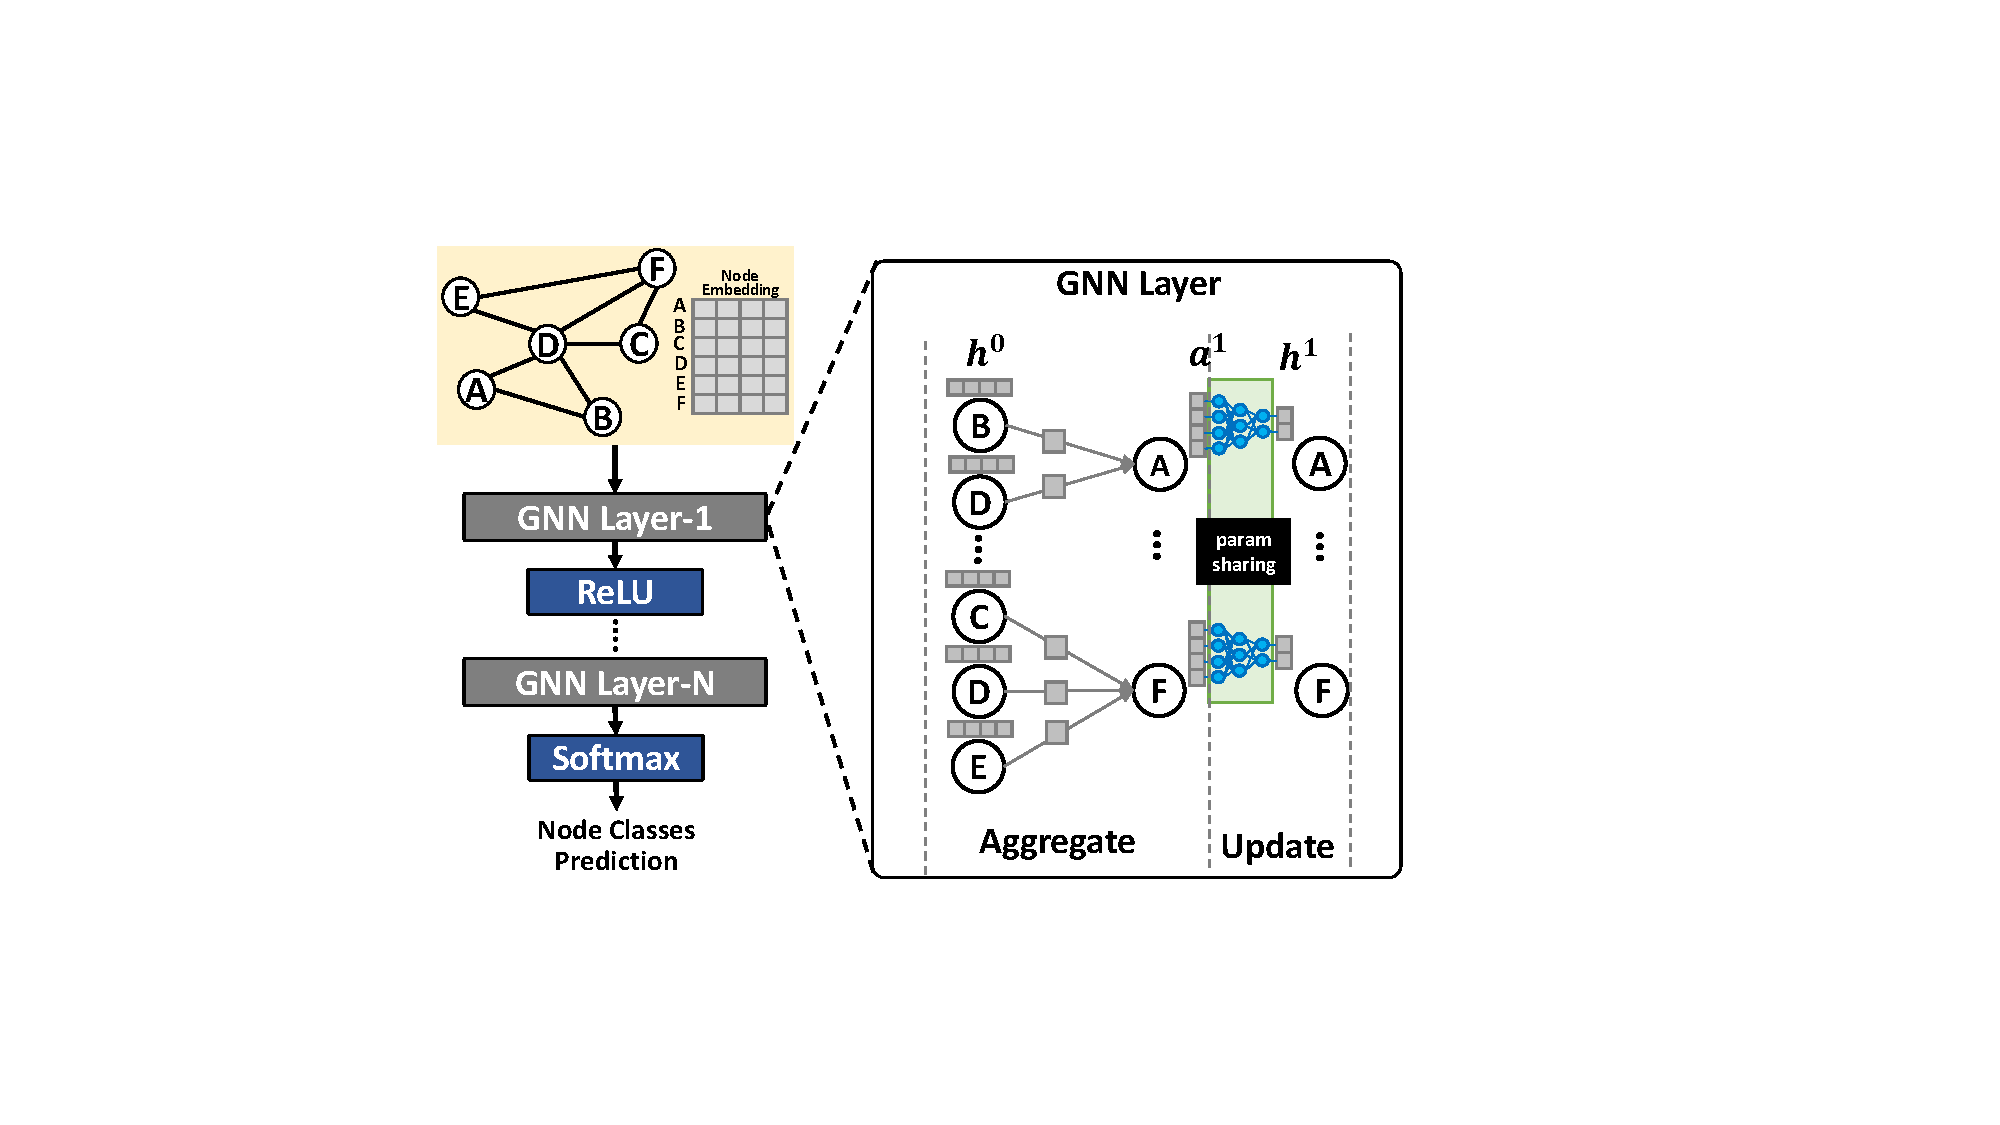
\includegraphics[width=0.6\textwidth]{images/gnn_background.pdf} % 调整宽度为单栏的合适比例
    \vspace{-5pt} % 可根据需要调整垂直间距
    \caption{GNN General Computation Flow.}
    \label{fig:gnn-computation-flow} % 修改标签以符合 LaTeX 的命名规范
\end{figure}

在经历多次聚合与更新的迭代过程(即多轮GNN层运算)后,我们将获得各节点的输出嵌入向量。该向量通常可用于基于图的深度学习下游任务,例如节点分类任务~\cite{kaspar2010graph, gibert2012graph, duran2017learning}和链接预测任务~\cite{chen2005link, kunegis2009learning, tylenda2009towards}。需特别说明的是,GNN输入层的初始节点嵌入既可以原始图数据集自带特征,还可以通过图嵌入算法生成(例如~\cite{grover2016node2vec, transE, duvenaud2015convolutional})。这类初始嵌入的生成过程独立于GNN模型的计算流程(即不参与隐藏层及输出层节点嵌入的计算)。

\subsection{图形处理器}
图形处理器(GPU)最初为加速图形渲染而设计,但其架构内在的大规模并行计算能力和高内存带宽,使其迅速发展成为通用并行计算(General-Purpose computing on GPUs, GPGPU)的主流平台,尤其在深度学习、科学计算等计算密集型领域取得了革命性的成功。对于同样有着巨大计算需求的图神经网络(GNN)而言,GPU自然成为了极具吸引力的加速硬件选择。

图形处理器(GPU)通过其大规模并行架构为GNN计算提供了强大的硬件基础。GPU包含数千个计算核心,组织在多个流式多处理器(SMs)中,并配备高带宽内存系统,以支持高吞吐量计算。要充分发挥其性能,关键在于有效利用GPU复杂的内存层次结构:这包括高速的寄存器和SM内部可编程的共享内存(Shared Memory),后者允许同一线程块内的线程高效协作。优化目标是最大化利用片上高速内存,并实现对全局内存的合并访问(Coalesced Access),即Warp内线程访问连续内存地址,以提升带宽利用率。

编程GPU通常采用如NVIDIA CUDA之类的模型。CUDA执行并行内核(Kernel),其执行单元是线程(Thread)。线程被组织成线程块(Block),块内线程可共享数据并同步。多个块组成线程网格(Grid)。硬件层面,线程以Warp(通常32个)为单位进行调度和执行,遵循单指令多线程(SIMT)模式。然而,GNN的不规则性给这种架构带来了挑战:图遍历导致的不规则内存访问难以合并;节点度的巨大差异造成负载不均衡;条件分支引发Warp发散,降低SIMT效率;聚合更新所需的原子操作则可能产生竞争瓶颈。因此,高效的GNN加速需要深入结合GNN的模型信息和GPU的硬件架构,根据不同的模型和硬件平台自适应做出深度优化。
% todo : 这里需要添加一张图,展示GPU内存模型和线程模型
%\begin{figure}:GPU内存模型和线程模型的图片
\subsection{图处理系统}
当前已有诸多图处理系统~\cite{khorasani2014cusha, Tigr, wang2016gunrock, liu2015enterprise, liu2019simd}致力于加速传统图算法。这些系统普遍采用顶点与节点编程抽象和边中心处理范式,并通过系统级优化来缓解计算不规则性(如负载不均衡)和内存访问不规则性(如非合并的全局内存访问)等问题。然而,将这些图处理系统扩展应用于GNN计算时却面临显著挑战。

首先,传统图处理中常见的算法优化策略对GNN往往收效甚微。以广度优先搜索为代表的图遍历算法依赖于对前驱节点(即活跃邻居)的迭代计算,因此催生了推拉式遍历~\cite{liu2015enterprise,liu2019simd}和前驱过滤~\cite{liu2015enterprise,liu2019simd,wang2016gunrock}等优化技术。但GNN在迭代过程中始终需要处理每个节点的全部邻居,这种固定规模的前驱访问特性使得传统前驱优化技术失去用武之地。

其次,图处理系统的优化技术必须经过针对性改造才能适配GNN特性。现有系统采用的节点与边处理机制~\cite{wang2016gunrock,liu2019simd}和基于分片的图表示方法~\cite{khorasani2014cusha}原本是针对单标量属性节点的优化方案。而GNN引入了高维嵌入向量这一新的并行维度,这就要求系统设计需要在更细粒度上重新权衡维度级并行性与节点嵌入局部性,而非简单沿用传统的节点级并行优化策略。

更为关键的是,现有图处理系统普遍缺乏支持GNN计算的核心功能模块。无论是基于神经网络的前向传播节点更新,还是复杂的反向梯度传播机制,在当前主流图系统~\cite{khorasani2014cusha, Tigr,wang2016gunrock,liu2015enterprise,liu2019simd,kyrola2012graphchi, x-stream}中均未实现。反观PyTorch~\cite{pytorch}和TensorFlow~\cite{tensorflow2015}等深度学习框架,其内置的自动微分功能可灵活支持各类模型架构的梯度计算。这种功能代差使得直接扩展图处理系统支持GNN面临巨大技术障碍,也促使我们选择基于深度学习框架开发全新的系统。

\subsection{深度学习框架}

目前学界和工业界已有提出了多种神经网络框架,包括TensorFlow~\cite{tensorflow2015}和PyTorch~\cite{pytorch}等。这些框架为传统深度学习模型提供了端到端的训练与推理支持,涵盖线性算子、卷积算子等多种神经网络算子。然而,这些算子主要针对图像等欧式数据进行了高度优化,缺乏对GNN中非欧式图数据的原生支持。要将这些神经网络框架扩展以支持处理高度不规则图数据的GNN计算,主要面临许多挑战。

首先,现有基于神经网络框架扩展的GNN计算平台~\cite{pyG,wang2019dgl}虽然注重不同GNN模型的编程通用性,但其底层运行时缺乏高效支持。以PyTorch Geometric(PyG)~\cite{pyG}为例,其采用CUDA实现的torch-scatter~\cite{torch-scatter}库作为图聚合操作的核心组件。该实现在处理中小规模稠密图时表现尚可,但当面对具有高维节点嵌入的大规模稀疏图时,由于内核设计沿用了图处理系统理念,过度依赖高开销的原子操作来支持节点嵌入传播,导致性能急剧下降。类似的可扩展性问题也出现在Deep Graph Library(DGL)~\cite{wang2019dgl}中:该系统对简单的求和聚合~\cite{GCNConv,SageConv}直接调用cuSparse~\cite{cusparse}的稀疏矩阵乘法(如\textit{csrmm2}),而对涉及边属性的复杂聚合~\cite{GINConv,GATConv}则采用自研CUDA内核,均存在性能瓶颈。

其次,主流的计算内核~\cite{pyG, wang2019dgl}采用硬编码实现,缺乏设计灵活性。从高层接口来看,用户仅能定义这些内核的外部组合方式,而无法根据已知的GNN模型架构特征、GPU硬件特性和图数据属性,对这些内核进行内部定制化优化。这种刚性设计难以适应不同规模图数据与节点嵌入维度的多样化应用场景,仍然存在巨大的优化空间。在Pytorch 2.0 中引入的torch.compile~\cite{torchCompile}通过即时编译(Just-In-Time Compilation,JIT)技术,允许用户在运行时对计算图进行优化。但是,主流的计算内核(如DGL~\cite{wang2019dgl})的许多核心功能依赖自定义 C++/CUDA 内核的操作,这些内核在编译时引发的图中断裂(Graph Breakage)会导致 JIT 优化失效,此外,这种通用的编译优化方法在处理GNN计算时仍然难以充分发挥 GPU 的硬件性能。

\subsection{本章小结}
本章旨在为后续深入探讨 GNN 加速技术奠定基础。我们首先阐述了图神经网络(GNN)的基本计算范式,包括其核心的聚合与更新流程,以及节点嵌入在多种下游任务中的关键作用。随后,深入剖析了图形处理器(GPU)的并行计算架构和内存体系,分析了其作为 GNN 加速硬件平台的巨大潜力,同时也指出了 GNN 固有的计算和访存不规则性给 GPU 高效利用带来的挑战。进一步地,本章回顾了传统的图处理系统,分析了其设计哲学和优化手段,并论证了这些系统难以直接、高效地扩展以支持 GNN 计算的根本原因,尤其是在处理高维特征向量和缺乏必要的神经网络及自动微分功能方面。最后,我们审视了当前主流深度学习框架在集成 GNN 支持时所面临的性能瓶颈,特别是底层稀疏计算内核的效率问题和硬编码实现带来的灵活性缺失,并初步探讨了如 torch.compile 等编译优化技术在这一背景下的潜力和局限。通过对这些基础技术及其相互作用的理解,为后续章节详细介绍针对 GNN 的算法、系统及硬件层面的加速策略提供了必要的背景知识和技术铺垫。



